
\documentclass[14pt]{bredelebeamer}
\usepackage{media9}
\usepackage{graphicx}
\usepackage{multimedia}
\usepackage{multicol}
\usepackage{subfig}
\usepackage{tikz}
\usepackage{setspace}
\usepackage[absolute,overlay]{textpos}

%%%%%%%%%%%%%%%%%%%%%%%%%%%%%%%%%%%%%%%%%%%%%%%%



\title[RUSIS @ OSU]{Take Me Out To The Ball Game}
% Titre du diaporama


\subtitle{An Analysis of the Home Run Surge in Major League Baseball}
% Sous-titre optionnel

\author{Leocadie Haguma, Rosalia Hernandez, Jacob Rojas\qquad}

\institute{RUSIS @ Oregon State University}

\date{August 23, 2018}
% Optionnel. La date, généralement celle du jour de la conférence

\subject{RUSIS @ OSU}
% C'est utilisé dans les métadonnes du PDF

\logo{

\includegraphics[scale=0.03]{images/OSU.png}
}



%%%%%%%%%%%%%%%%%%%%%%%%%%%%%%%%%%%%%%%%%%%%%%%%%%%%%%%%%%%%%%%%%%%%%
\begin{document}
%\onehalfspacing

\begin{frame}
  \titlepage
\end{frame}


\begin{frame}{Table of Contents}
  \tableofcontents
\end{frame}


\section{History}
\begin{frame}{History}
\begin{columns}

\begin{column}{0.7\textwidth}
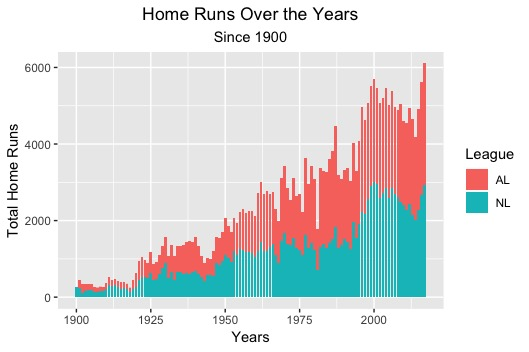
\includegraphics[scale = 0.42]{Graphs/Rplot}
\end{column}

\begin{column}{0.5\textwidth}

Historical Events (Getz 2009)

Notable Rule Changes:

\begin{itemize}
\begin{small}
\item 1920's : Babe Ruth
\item 1945 - 1950: World War II
\item 1969: Pitcher's Mound Lowered 5 inches
\item 1973: Pitcher's designated batter
\item 1981: Strike Canceled 713 Games
\item 1994: The "Great Strike" 
%World Series Canceled
\item 2000's: Steroids
\item 2015: ?
\end{small}
\end{itemize}
\end{column}
\end{columns}
\end{frame}


\begin{frame}

\begin{block}{\large Our Problem}

{\setstretch{1.5}\large There is an increasing trend of home runs within Major League Baseball between the 2015 to 2017 seasons. We plan to explore why and how this trend occurred.\\}

\end{block}

 

\end{frame}


\begin{frame}{Speculation}


\includegraphics[scale = 0.8]{images/Verlander.PNG}

\end{frame}


\section{Previous Work}


\begin{frame}{Official Investigation}

\begin{block}{Report of the Committee Studying Home Run Rates in Major League Baseball (Albert, 2018)}

The Scientists (Albert et. al 2018): 
\begin{itemize}
\begin{small}
\item Jim Albert, Professor of Statistics at Bowling Green State University
\item Jay Bartroff, Professor of Mathematics and the Graduate Vice-Chair for Statistics at USC
\item Roger Blandford, Luke Blossom Professor in the School of Humanities at Standford University
\item Dan Brooks, Researcher and Co-Organizer of Saberseminar
\item Josh Derenski, Statistics PhD Student in the USC Marshall School of Business
\item Larry Goldstein, Professor of Mathematics at the University of Southern California
\item Anette (Peko) Hosoi, Neil and Jane Pappalardo Professor of Mechanical Engineering and Mathematics at MIT
\item Gary Lorden, Professor Emeritus of Mathematics at Caltech
\item Alan Nathan (Chair), Professor Emeritus of Physics at the University of Illinois at Urbana-Champaign
\item Lloyd Smith, Professor in the School of Mechanical and Materials Engineering at Washington State University
\end{small}
\end{itemize}
\end{block}
\end{frame}

\begin{frame}{Terms}
  \begin{columns}
   \begin{column}{0.5\textwidth}
      \begin{block}{Launch Angle}
      The angle from when the ball hits the bat and flies 		into the outfield.
      \end{block}
    \end{column}
  \begin{column}{0.5\textwidth}
  \begin{block}{Exit Velocity} 
  The initial speed of the ball immediately after being hit 	by the bat.
  \end{block}
  \end{column}
  \end{columns}
  
%\begin{center}
%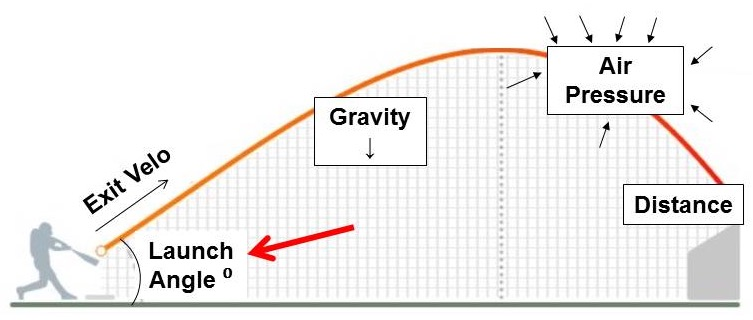
\includegraphics[scale = 0.25]{images/LaunchAExitV-DarenWillman} 
%\end{center}

\begin{figure}[]
\centering
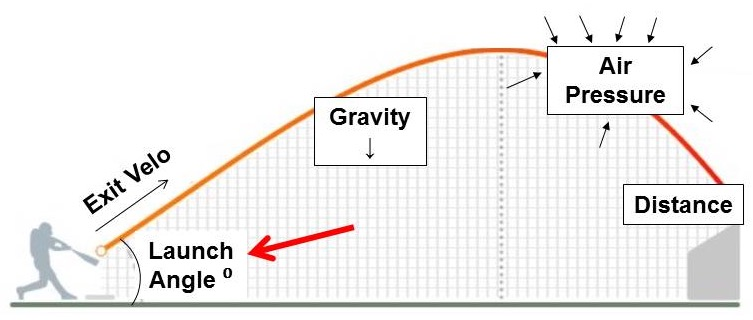
\includegraphics[scale = 0.27]{images/LaunchAExitV-DarenWillman}
\caption{Image by Daren Willman, Director of R\&D at MLB}
\label{figure:DKinflation}
\end{figure}


  \begin{alertblock}{Red Zone}
  The majority of home runs are within the parameters of an 	exit velocity between 90 to 115 mph, and 15 to 45 		degree launch angle.
  \end{alertblock}
\end{frame}

\begin{frame}{Official Investigation}
  \begin{block}{Their initial thoughts about home runs}
    \begin{itemize}
      \item Concentration of home runs among players
      \item Concentration of home runs among ballparks 
      \item Changes in pitching strategy
      \item Changes in batting strategy
      \item Characteristics of home runs
    \end{itemize}
  \end{block}
    \begin{block}{Committee Findings}
    \begin{itemize}
    \item The probability of hitting a ball into the "Red 		Zone" did not change.
    \item The probability of hitting a ball into the "Red 		Zone" and making a home run did change.
    \end{itemize}
  \end{block}
\end{frame}

\begin{frame}{The Red Zone}

\begin{columns}
\begin{column}{0.5\textwidth}
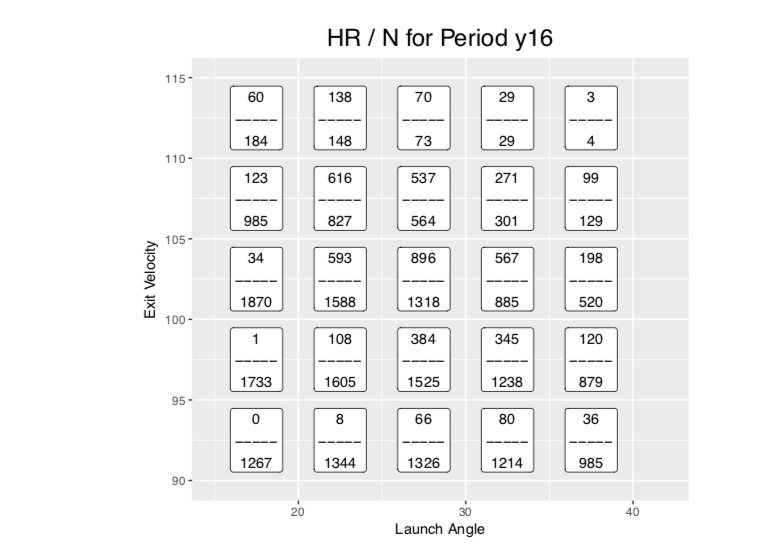
\includegraphics[scale = 0.6, trim = 2.2cm 0 0 0]{images/Committee_2016}
\end{column}
\begin{column}{0.6\textwidth}
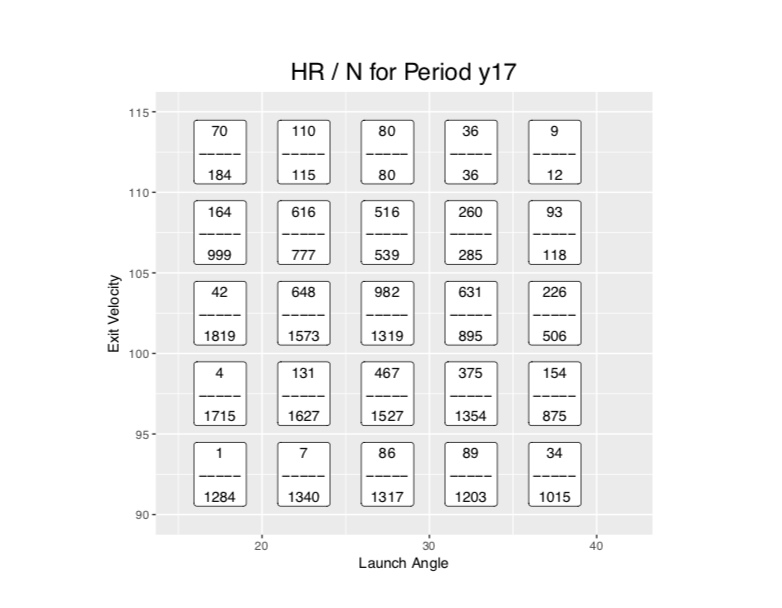
\includegraphics[scale = 0.62, trim = 0.7cm 0 0 0]{images/Committee_2017}
\end{column}
\end{columns}
\begin{small}
\begin{center}
Images by The Committee of Scientists studying the home run surge in the MLB
\end{center}
\end{small}

\end{frame}


\begin{frame}{Official Committee}

\begin{block}{Exploring the factors that affect the carry of a baseball}

Temperature:
  \begin{itemize}
    \item Examined home run rates against temperature for 		open stadiums and for closed stadiums. 
    \item They founds similar trends through the seasons 		examined (2015-2017).
    \item Conclusion: The home run surge could not be 		explained by the effect of temperature.
  \end{itemize}

The Ball :
  \begin{itemize}
    \item Examining the manufacturing process of MLB 		baseballs required a trip to Rawlings Sporting Goods, 		the official MLB baseball manufacturer, located in 		Costa Rica.
    \item Rawlings Sporting Goods measure the baseball's 		weight, circumference, compression, coefficient of 		restitution(COR).
    \item Need more information
  \end{itemize}
\end{block}
\end{frame}

\begin{frame}{Official Committee}

\begin{block}{More testing}
\begin{itemize}
\item Sports Science Laboratory at Washington State University
\begin{itemize}
\item UMass Lowell Baseball Research Center 2013-2017 
\item MLB, authenticated, 2012-2017
\item Impact testing, aerodynamic testing
\item Other Properties: seam heights, center of gravity, surface roughness
\end{itemize}
\item Analysis of StatCast Trajectories 
\end{itemize}
\end{block}
\begin{block}{Conclusions}
The baseball has shown changes in its aerodynamic properties that are not currently being measured or recorded. Since the baseballs are being made within the parameters set by the MLB, there is not evidence that supports the claim that the baseball has physically changed (Albert, 2018).
\end{block}
\begin{block}{Some Recommendation}
\begin{itemize}
\item Implement new parameters to measure and monitor the characteristics of the baseballs that affect carry.
\item Monitor the baseball storage climate.
\end{itemize}
\end{block}
\end{frame}

\begin{frame}{Fivethiryeight.com}
\begin{block}{The Researchers}

	\begin{itemize}
		\item A data journalism blog created by Nate Silver who is an American statistician.
		\item Long history of predictive analytics successes in sports and politics.
	\end{itemize}
\end{block}  
\begin{block}{What did the researchers do?}

	\begin{itemize}
        \item Used a Computed Tomography (CT) scan to X-ray baseballs 
        \begin{itemize}
        \item This looked at the density of the rubber lining of the ball 
        \end{itemize}
		\item Used a Thermogravimetric testing for a Chemical Composition of the ball.
        \begin{itemize}
        \item This looked at identifying the chemical changes in the rubber lining   
        \end{itemize}
	\end{itemize}
\end{block}  
\end{frame}

\begin{frame}{Findings}
\begin{block}{Discoveries}
\begin{itemize}
\item The baseballs used by the MLB prior to 2015 were more dense and weighed more than the ones being used now. 
\end{itemize}

\end{block}

\begin{columns}
\begin{column}{0.3\textwidth}
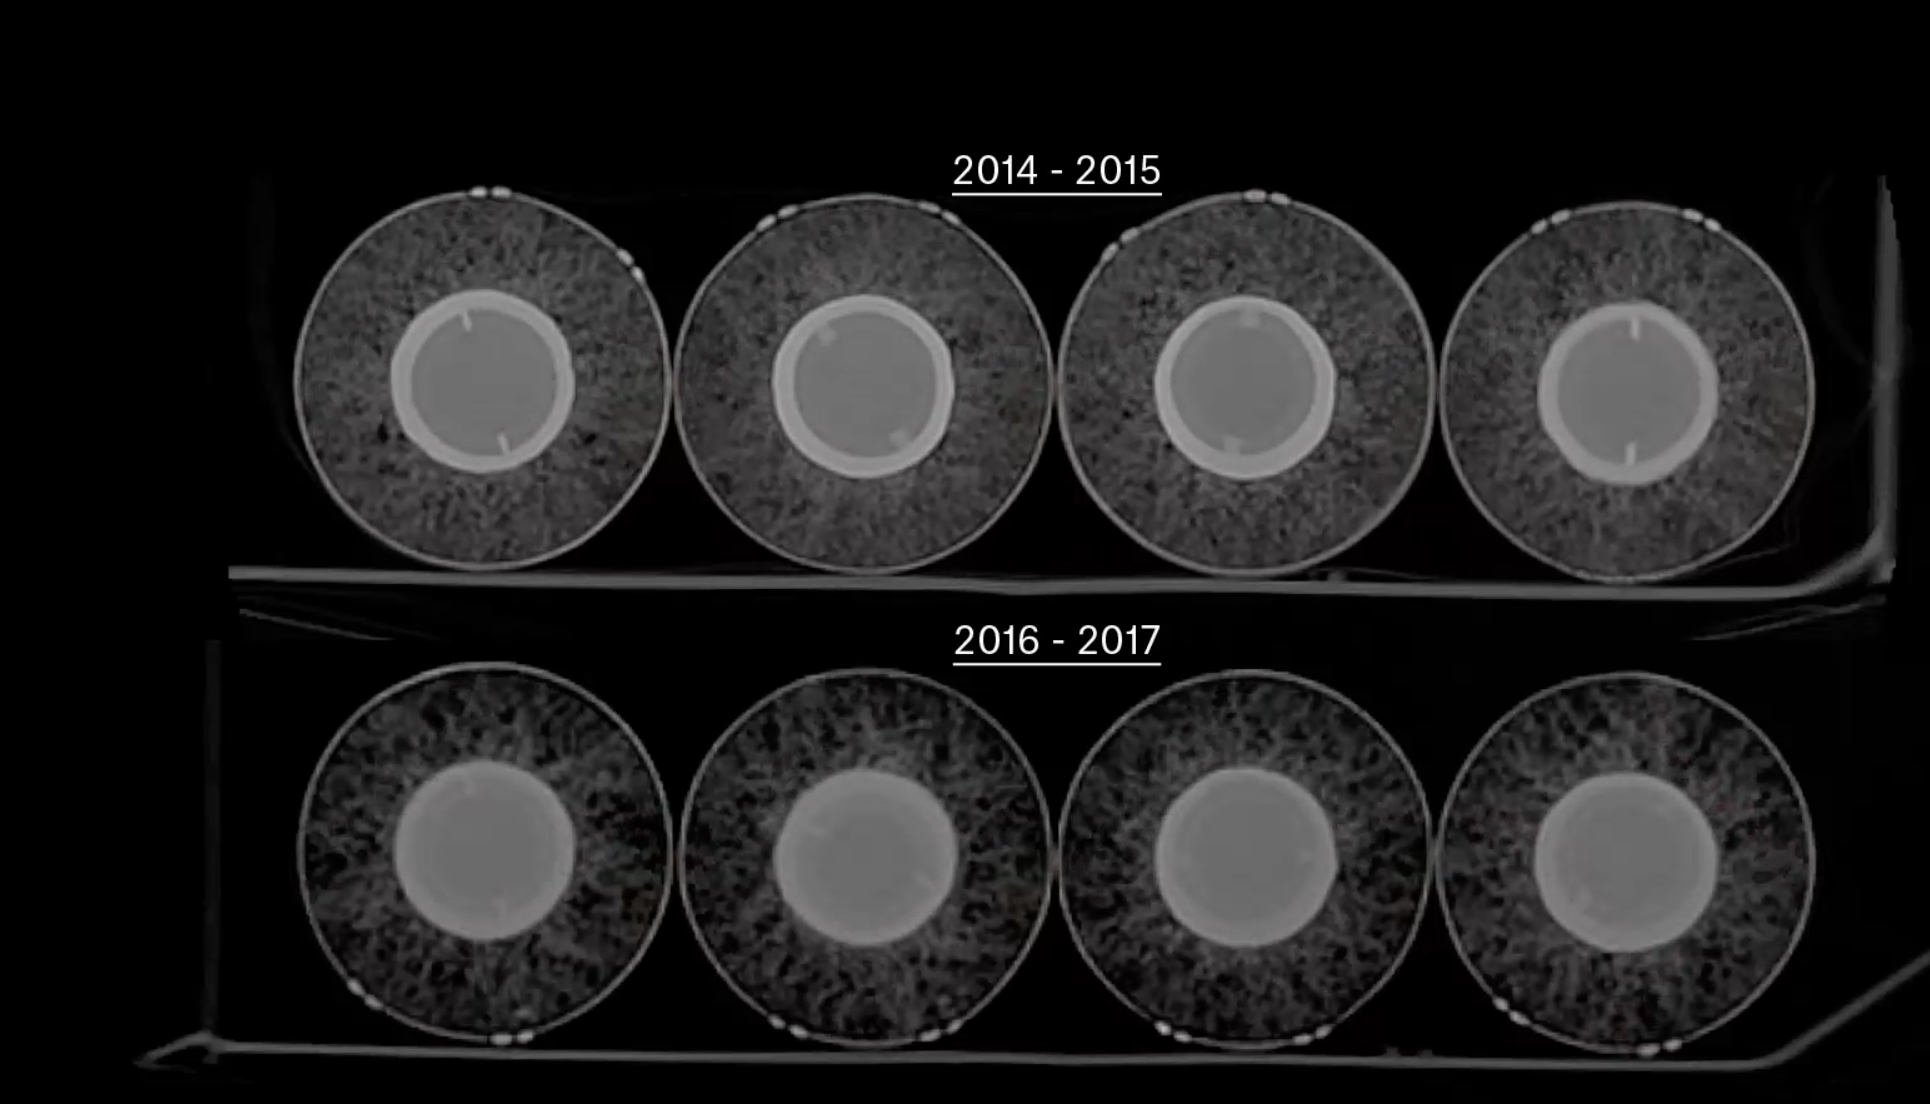
\includegraphics[scale = 0.07]{images/all_xray}
\end{column}
\begin{column}{0.4\textwidth}
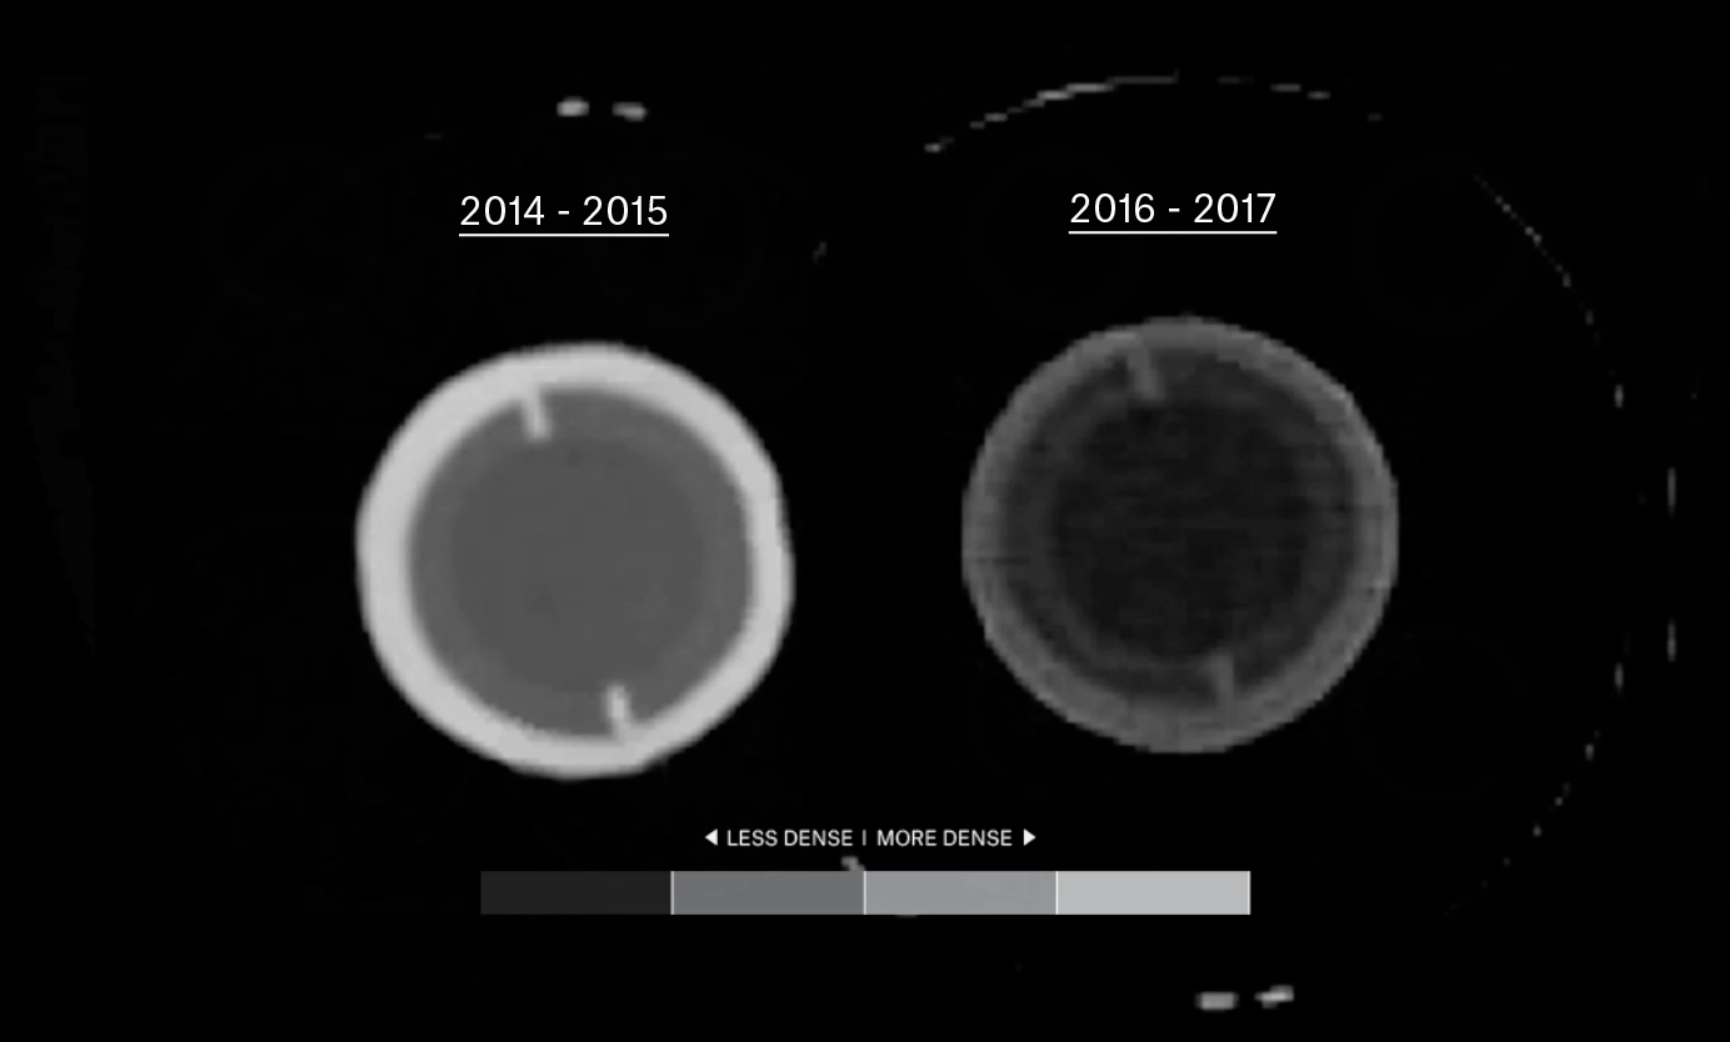
\includegraphics[scale = 0.075]{images/density_balls}
\end{column}
\end{columns}
\centering
Image by fivethirtyeight.com

\end{frame}


\begin{frame}{Fivethiryeight.com Conclusions}


\begin{block}{Findings}
	\begin{itemize}
    	\item The chemical composition of the core of the baseball changed
        \item The baseball was "bouncier"
        \item The rubber portion of the core was less dense
        \item The entire baseball was now 0.5 grams lighter 
    \end{itemize}
\end{block}
\begin{block}{Conclusion}
	\begin{itemize}
    	\item These changes to the ball could only account for 25\% increase in home runs
        \item The surge was a 46\% increase home runs
    \end{itemize}
\end{block}

\end{frame}


\section{Our Work}

\begin{frame}

\begin{block}{\large Our Story}
{\setstretch{2} \large We believe the most unexplored area of the surge is the players themselves.\\}

\end{block}	

\end{frame}

%\begin{frame}{StatCast}

%\movie[scale = 0.5]{images/statcastphoto}{Statcast}
%\end{frame}

\begin{frame}{Difficulty in Collecting Data}
\begin{block}{Initial data collection}
\begin{itemize}
\item Initial data gathering conducted on MLB stats website. Interface built for viewing, not scraping.
\item Gathering data through MLB proved to be inefficient.
%\item Discovery of Lahman database allowed us to begin analysis with more data.
%\item Finding and learning R package \textit{Baseballr} would give us access to pitching data dating back to 2010. 
\end{itemize}
\end{block}
\end{frame}

%\begin{frame}{Data Collection}
%\begin{block}
%\begin{itemize}
%    	\item Baseball Savant: StatCast measurements (pitch speed, exit velocity, etc.)
%        \item Lahman: general player info (age, height, weight)
%\end{itemize}
%\end{block}
%\end{frame}


\begin{frame}{Data Collection}
\begin{block}{Baseball Savant}
\begin{itemize}
\item Statcast measurement 
\item Pitchfx data (Release speed, Type of pitch, etc.)
\item Hitfx data (Exit velocity, Launch angle, etc. )
\end{itemize}
\end{block}
\begin{block}{Lahman Database}
\begin{itemize}
\item General MLB information 
\item Age, Height, weight
\item Teams, Leagues (NL and AL)
\end{itemize}
\end{block}

\end{frame}

\begin{frame}{Data Organization}
\begin{block}{\large Joining Databases}
\begin{itemize}
\item \large Statcast pitching data back to 2004. Over 8 million total pitches.
\item \large Lahman data of player information dating back to beginning of baseball.
\item \large Joining of databases to have complete picture. Using unique batter IDs and names in combination with \textit{Baseballr} player lookup function, databases could be joined.
\end{itemize}
\end{block}
\end{frame}

\begin{frame}
\begin{block}{\large Good Data}
\large \textit{"Data is good, only if it is good data"} -- Dr. Javier Rojo
\end{block}
\end{frame}

\begin{center}
\includemedia[
width = 8cm, height = 8cm,
addresource = Statcast.mp4,
transparent, activate = pagevisible, 
flashvars = {
source = Statcast.mp4
&autoplay = true
&loop = false
}
]{}{VPlayer.swf}
\end{center}

\begin{frame}{Bryce Harper's Home run}
\begin{center}
\includemedia[
width = 9cm, height = 9cm,
addresource = Harper.mp4,
transparent, activate = pagevisible, 
flashvars = {
source = Harper.mp4
&autoplay = true
&loop = false
}
]{}{VPlayer.swf}
\end{center}
\end{frame}

%\begin{frame}
%\begin{block}{\large Data Cleaning}
%	\begin{itemize}
 %   \item \large Large database needs refining to examine parameters important to our investigation
 %   \item \large Referencing a Lahman table of pitchers as technique to remove pitchers
 %   \item \large Filtering by debut date to isolate rookies
 %   \item \large Filtering by event to isolate home runs
  %  \end{itemize}
%\end{block}
%\end{frame}

%\begin{frame}{Data Organization}
%\centering
%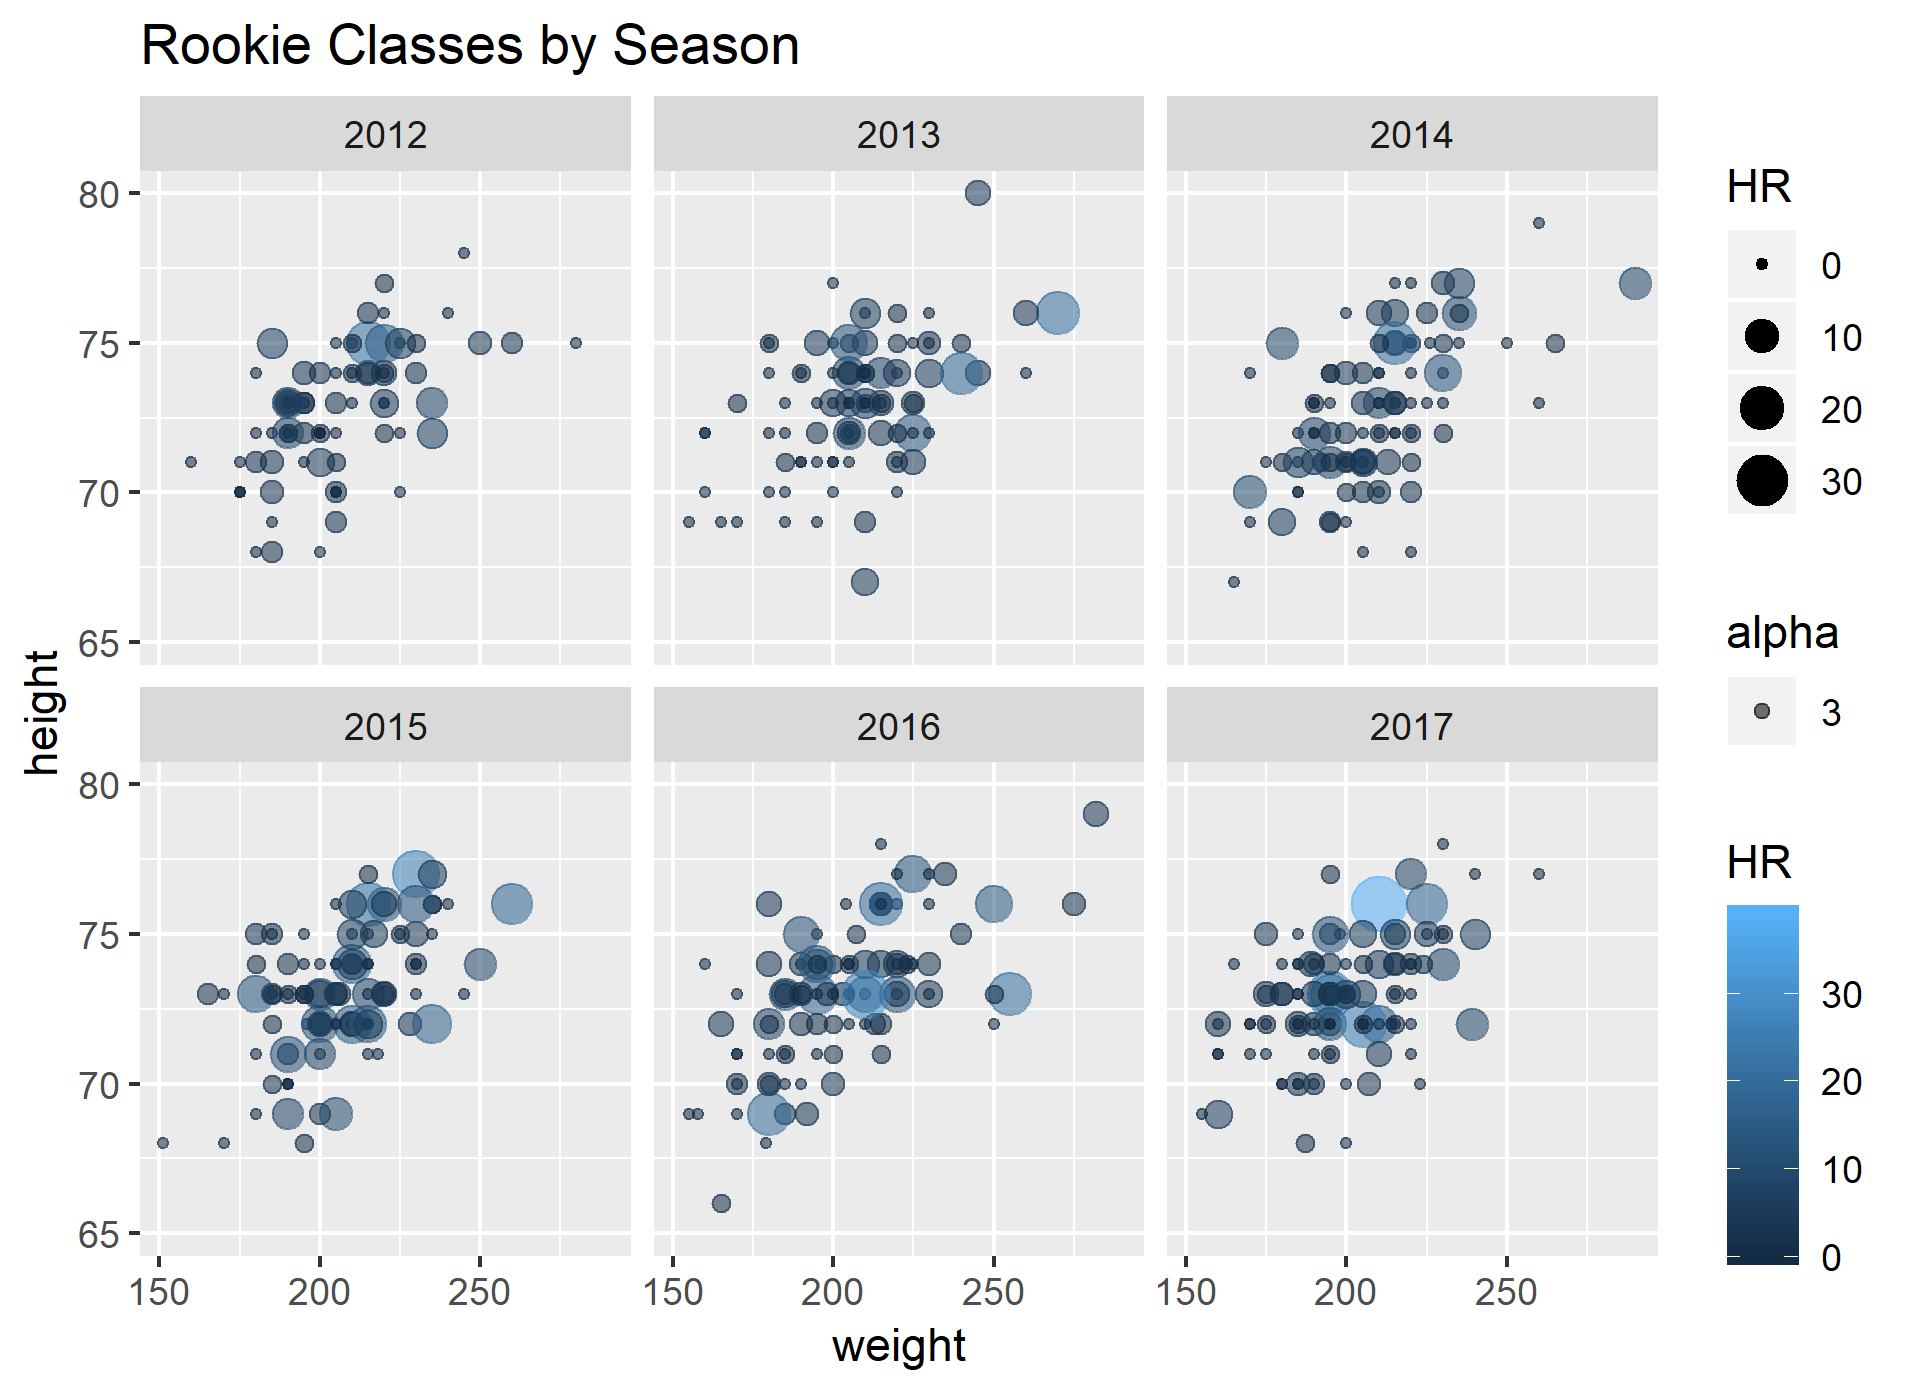
\includegraphics[scale=0.5]{Graphs/rookie_no_pitcher.png}
%\end{frame}

%\begin{frame}{Data Organization}
%    \centering
%     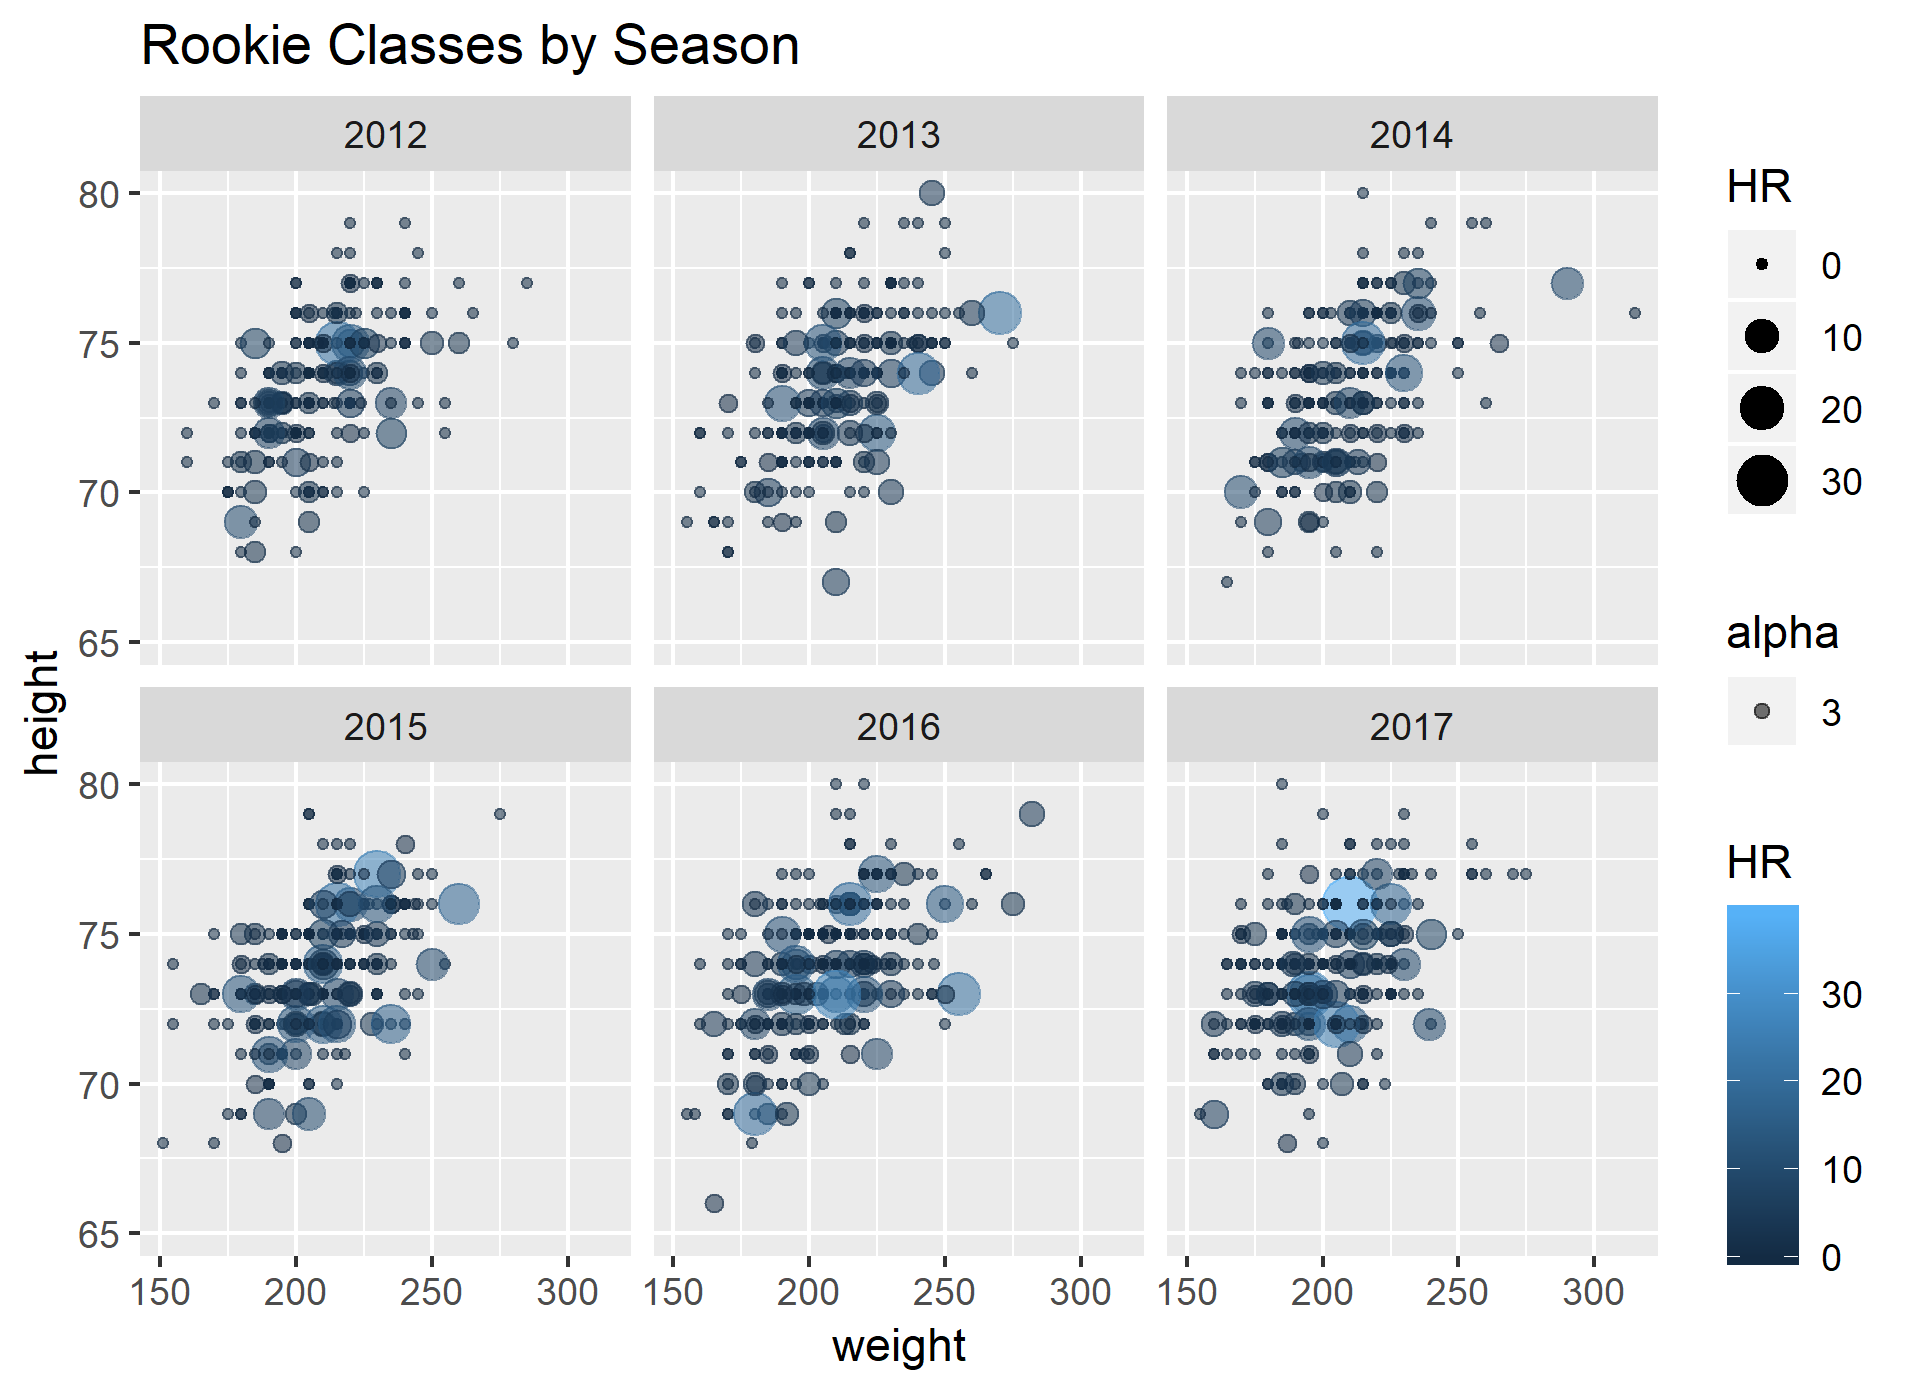
\includegraphics[scale = 0.5]{Graphs/rookie_with_pitcher.png}
%\end{frame}
  		

\begin{frame}
\begin{block}{\large Players}
{\setstretch{1.5} \large Our investigation focused on how the players themselves were affecting the increase in home runs. We decided to look at the following variables for this:\\}
	\begin{itemize}
    	\item \large Age
        \item \large Height and Weight
        \item \large Pitchers
        \item \large New MLB players (Rookies)
    \end{itemize}
\end{block}
\end{frame}


\begin{frame}{Age}
	\begin{center}
    	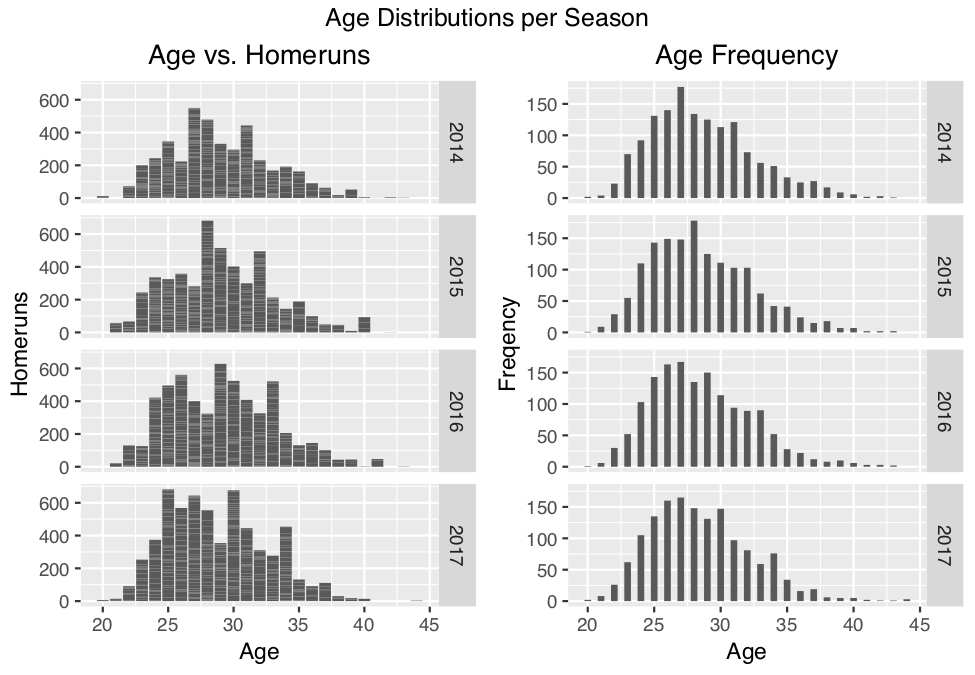
\includegraphics[scale = 0.6]{Graphs/homerun_ages.png}
    \end{center}
\end{frame}


\begin{frame}{Heights of All MLB Players}
	\begin{center}
    	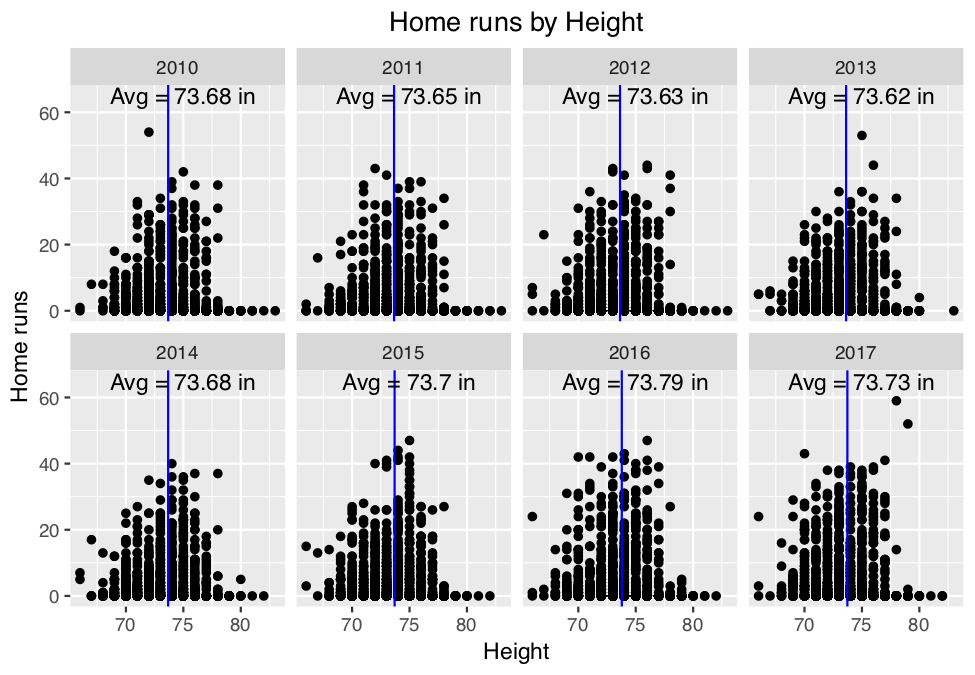
\includegraphics[scale = 0.6]{Graphs/wh_with_pitchers.png}
    \end{center}
\end{frame}

\begin{frame}{Weights of All MLB Player}
	\begin{center}
    	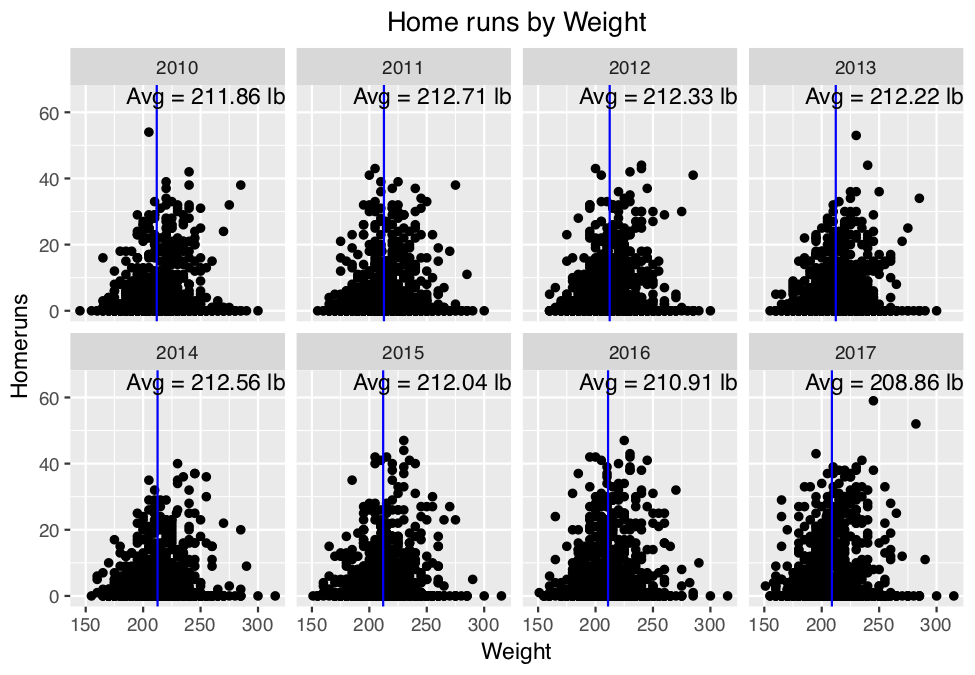
\includegraphics[scale = 0.6]{Graphs/wh_with_pitchers_1.png}
    \end{center}
\end{frame}

\begin{frame}{Heights of MLB Batters}
	\begin{center}
    	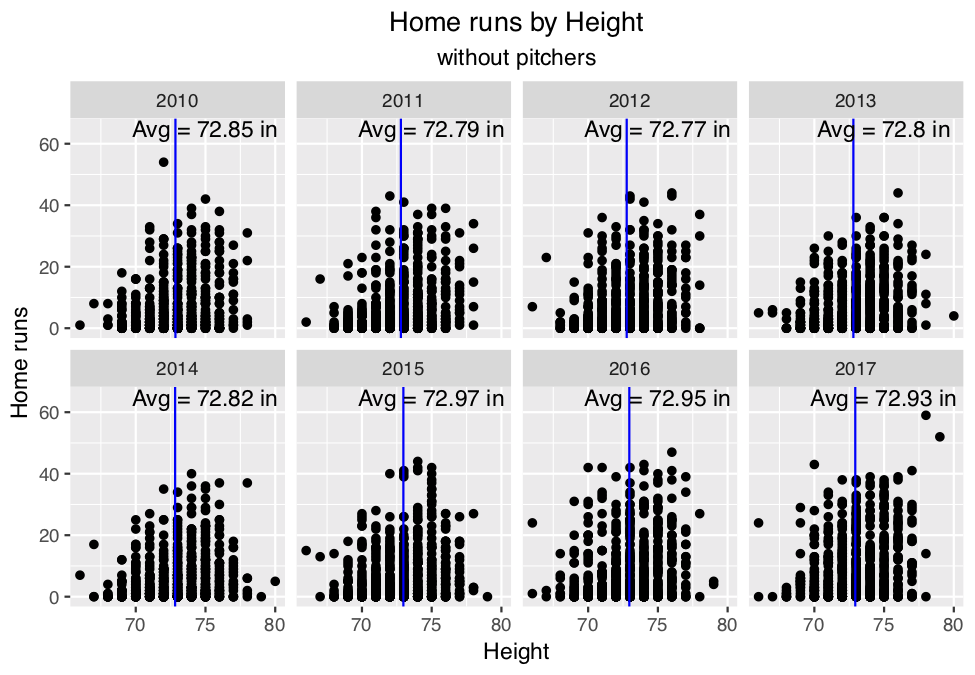
\includegraphics[scale = 0.6]{Graphs/h_wihout_pitchers.png}
    \end{center}
\end{frame}

\begin{frame}{Weights of MLB Batters }
	\centering
    	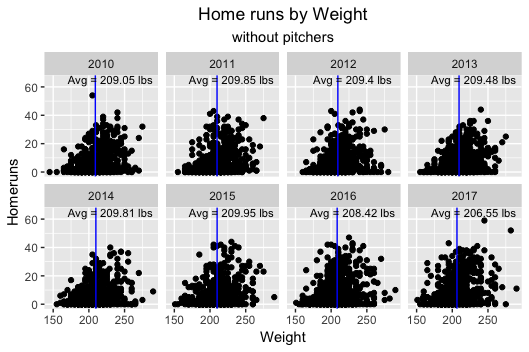
\includegraphics[scale = 0.55]{Graphs/weightnopitch.png}
    
\end{frame}

\begin{frame}{All New MLB Players (Rookies)}
Is the incoming class of MLB hitters affect by the home run surge?
	\begin{center}
    	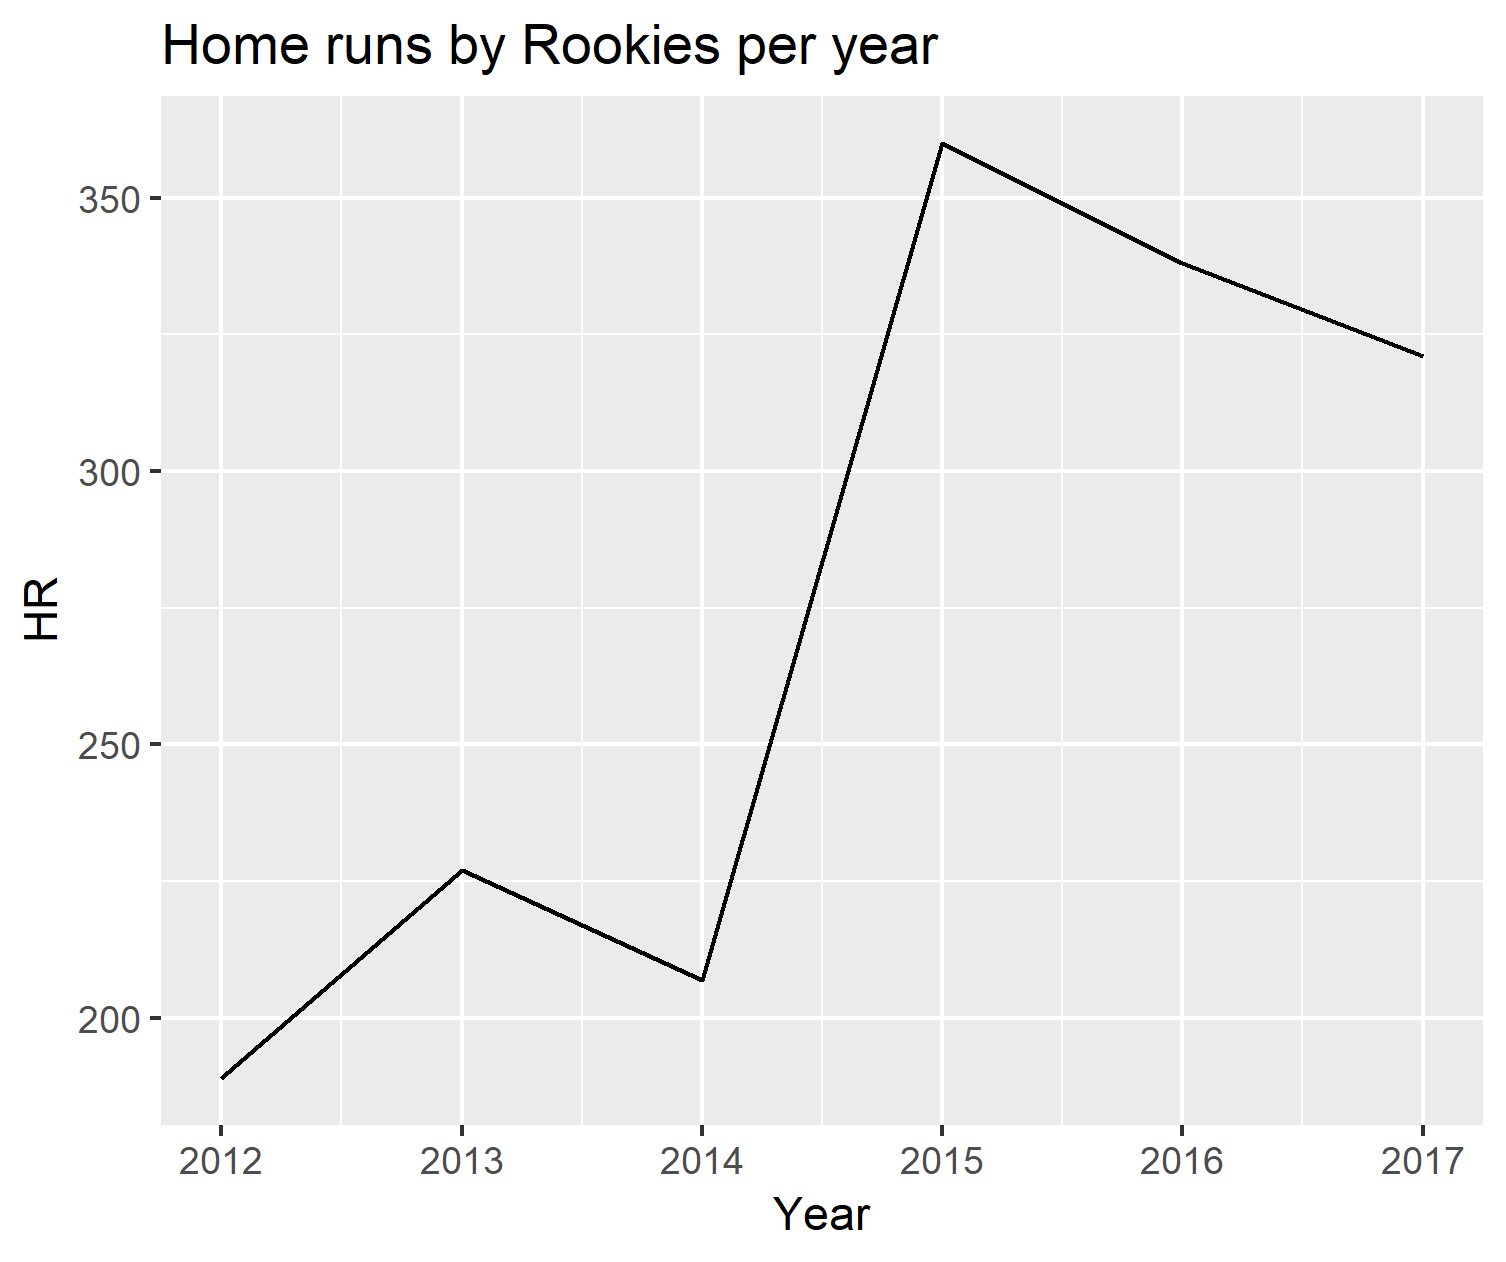
\includegraphics[scale = 0.5]{Graphs/rookie_hrs.png}
    \end{center}
\end{frame}


\begin{frame}{New MLB Players (Rookies) cont...}
	\begin{center}
    	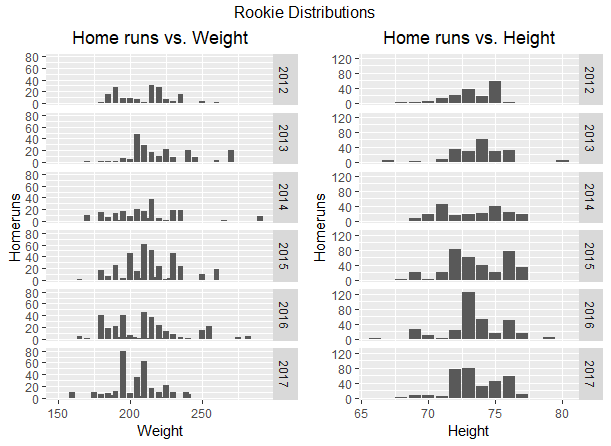
\includegraphics[scale = 0.6, trim=0 0 0 0]{Graphs/rookie_no_pitch_weight_height.png}
     \end{center}
\end{frame}


\begin{frame}{Pitchers}
	\begin{center}
    	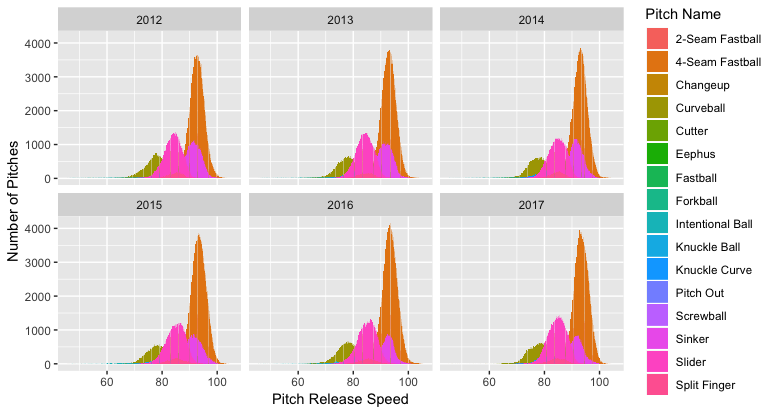
\includegraphics[scale = 0.4, trim=0 0 0 0]{Graphs/pitches.png}
     \end{center}
\end{frame}


\begin{frame}{Logistic Regression}
\begin{alertblock}{Logistic Regression}
\begin{itemize}
\item A logistic regression allows us to analyze the impact of a group of variables on a response variable (Home run = 0,1). 
    \end{itemize}
    
\end{alertblock}
	
\begin{block}{Variables:}
	\begin{multicols}{3}
	\begin{itemize}
		\item Release Speed
        \item Launch Speed
        \item Weight
        \item Height
        \item Stand
        \item Age
        \item Pitch throw
        \item Interaction of height and weight
        \item Multiple logistic regressions: Pre/Post 2015, Post 2015 with launch speed
	\end{itemize}
    \end{multicols}
    \end{block}
\end{frame}

\begin{frame}{Significance}
\begin{table}[]
\begin{tabular}{|
>{\columncolor[HTML]{DAE8FC}}l |
>{\columncolor[HTML]{DAE8FC}}l |
>{\columncolor[HTML]{DAE8FC}}l |
>{\columncolor[HTML]{DAE8FC}}l |
>{\columncolor[HTML]{DAE8FC}}l |
>{\columncolor[HTML]{DAE8FC}}l |}
\hline
\multicolumn{6}{|c|}{\cellcolor[HTML]{B0D0FD}\textbf{Pre-2015 Logistic Regression}}                                                                                                                                              \\ \hline
\multicolumn{1}{|c|}{\cellcolor[HTML]{DAE8FC}}              & \multicolumn{1}{c|}{\cellcolor[HTML]{DAE8FC}Estimate}   & \multicolumn{1}{c|}{\cellcolor[HTML]{DAE8FC}Std. Error} & z value & Pr(\textgreater{}|z|) & Significance \\ \hline
\multicolumn{1}{|c|}{\cellcolor[HTML]{DAE8FC}Release Speed} & \multicolumn{1}{c|}{\cellcolor[HTML]{DAE8FC}-0.0063463} & \multicolumn{1}{c|}{\cellcolor[HTML]{DAE8FC}0.0012061}  & -5.262  & <<0.001              & ***          \\ \hline
Weight                                                      & \multicolumn{1}{c|}{\cellcolor[HTML]{DAE8FC}0.0094586}  & \multicolumn{1}{c|}{\cellcolor[HTML]{DAE8FC}0.0005333}  & 17.737  &  <<0.001       & ***          \\ \hline
Height                                                      & 0.0500789                                               & 0.0049122                                               & 10.195  &  <<0.001       & ***          \\ \hline
Age                                                         & 0.0116417                                               & 0.0025300                                               & 4.601   & <<0.001              & ***          \\ \hline
Stand\_R                                                    & 0.0908204                                               & 0.0147309                                               & 6.165   & <<0.001              & ***          \\ \hline
Pitcher\_R                                                  & 0.0441629                                               & 0.0162320                                               & 2.721   & 0.00651               & **           \\ \hline
\end{tabular}
\end{table}
\begin{block}{Significance codes}
	\begin{itemize}
		\item 0 '***' 0.001 '**' 0.01 '*' 0.05 '.' 0.1 ' ' 1
	\end{itemize}
    \end{block}
\end{frame}

\begin{frame}{Significance cont...}
\begin{table}[]
\begin{tabular}{|
>{\columncolor[HTML]{DAE8FC}}l |
>{\columncolor[HTML]{DAE8FC}}l |
>{\columncolor[HTML]{DAE8FC}}l |
>{\columncolor[HTML]{DAE8FC}}l |
>{\columncolor[HTML]{DAE8FC}}l |
>{\columncolor[HTML]{DAE8FC}}l |}
\hline
\multicolumn{6}{|c|}{\cellcolor[HTML]{B0D0FD}\textbf{Post-2015 Logistic Regression}}                                                                                                                                             \\ \hline
\multicolumn{1}{|c|}{\cellcolor[HTML]{DAE8FC}}              & \multicolumn{1}{c|}{\cellcolor[HTML]{DAE8FC}Estimate}   & \multicolumn{1}{c|}{\cellcolor[HTML]{DAE8FC}Std. Error} & z value & Pr(\textgreater{}|z|) & Significance \\ \hline
\multicolumn{1}{|c|}{\cellcolor[HTML]{DAE8FC}Release Speed} & \multicolumn{1}{c|}{\cellcolor[HTML]{DAE8FC}-0.0058135} & \multicolumn{1}{c|}{\cellcolor[HTML]{DAE8FC}0.0013788}  & -4.216  & <<0.001               & ***          \\ \hline
Weight                                                      & \multicolumn{1}{c|}{\cellcolor[HTML]{DAE8FC}0.0090255}  & \multicolumn{1}{c|}{\cellcolor[HTML]{DAE8FC}0.0005521}  & 16.347  & <<0.001       & ***          \\ \hline
Height                                                      & 0.0403999                                               & 0.0053456                                               & 7.558   & <<0.001              & ***          \\ \hline
Age                                                         & -0.0038989                                              & 0.0022585                                               & -1.726  & 0.0843                & .            \\ \hline
Stand\_R                                                    & 0.0703056                                               & 0.0167903                                               & 4.187   & <<0.001              & ***          \\ \hline
Pitcher\_R                                                  & 0.0792483                                               & 0.0189381                                               & 4.185   & <<0.001              & ***          \\ \hline
\end{tabular}
\end{table}
\begin{block}{Significance codes}
	\begin{itemize}
		\item 0 '***' 0.001 '**' 0.01 '*' 0.05 '.' 0.1 ' ' 1
	\end{itemize}
    \end{block}
\end{frame}

\begin{frame}{Significance cont...}
\begin{table}[]
\begin{tabular}{|
>{\columncolor[HTML]{DAE8FC}}l |
>{\columncolor[HTML]{DAE8FC}}l |
>{\columncolor[HTML]{DAE8FC}}l |
>{\columncolor[HTML]{DAE8FC}}l |
>{\columncolor[HTML]{DAE8FC}}l |
>{\columncolor[HTML]{DAE8FC}}l |}
\hline
\multicolumn{6}{|c|}{\cellcolor[HTML]{B0D0FD}\textbf{Post-2015 Logistic Regression With Added Variables}}                                                                                                                        \\ \hline
\multicolumn{1}{|c|}{\cellcolor[HTML]{DAE8FC}}              & \multicolumn{1}{c|}{\cellcolor[HTML]{DAE8FC}Estimate}   & \multicolumn{1}{c|}{\cellcolor[HTML]{DAE8FC}Std. Error} & z value & Pr(\textgreater{}|z|) & Significance \\ \hline
\multicolumn{1}{|c|}{\cellcolor[HTML]{DAE8FC}Release Speed} & \multicolumn{1}{c|}{\cellcolor[HTML]{DAE8FC}-3.763e-02} & \multicolumn{1}{c|}{\cellcolor[HTML]{DAE8FC}1.518e-03}  & -24.789 & \textless <<0.001       & ***          \\ \hline
Launch Speed                                                & 1.960e-01                                               & 1.485e-03                                               & 131.957 & \textless <<0.001       & ***          \\ \hline
Weight                                                      & \multicolumn{1}{c|}{\cellcolor[HTML]{DAE8FC}1.633e-02}  & \multicolumn{1}{c|}{\cellcolor[HTML]{DAE8FC}1.520e-02}  & 1.075   & 0.282563              &              \\ \hline
Height                                                      & 4.729e-02                                               & 4.350e-02                                               & 1.087   & 0.277006              &              \\ \hline
Age                                                         & 1.711e-02                                               & 2.452e-03                                               & 6.979   & <<0.001              & ***          \\ \hline
Stand\_R                                                    & -6.822e-02                                              & 1.823e-02                                               & -3.741  & <<0.001              & ***          \\ \hline
Pitcher\_R                                                  & 8.883e-02                                               & 2.056e-02                                               & 4.320   & <<0.001              & ***          \\ \hline
Weight:Height                                               & -2.417e-04                                              & 2.070e-04                                               & -1.168  & 0.242937              &              \\ \hline
\end{tabular}
\end{table}
\begin{block}{Significance codes}
	\begin{itemize}
		\item 0 '***' 0.001 '**' 0.01 '*' 0.05 '.' 0.1 ' ' 1
	\end{itemize}
    \end{block}
\end{frame}


\section{Conclusions}

\begin{frame}{Conclusions}
\begin{block}{\large Summary}
\begin{itemize}
\item History of home runs in MLB tell us a story
\item Widespread speculations
\item Previous work 
	\begin{itemize}
	\item Official MLB committee: changes in drag coefficient
    \item fivethirtyeight: changes in chemical composition
	\end{itemize}
\item Our work revealed that the change in players had no effect on the surge in home runs. 
\item Our logisitic regression emphasized that the surge affected all players and that launch speed is a better proxy for strength.
\end{itemize}
\end{block}
\begin{alertblock}{Further Analysis}
\begin{itemize}
\item Further investigation to validate the change in significance of the handedness of the pitcher could provide more information on the home run surge. 
\end{itemize}

\end{alertblock}
\end{frame}



\begin{frame}{Acknowledgment}
\large This work was supported through NSA grant
number H98230-18-1-0009 and NSF grant
DMS-1731082, to Dr. Javier Rojo PI, through
the RUSIS @ Oregon State University.
\end{frame}

\end{document}